% ============================================================================
% Homework 2 -- Solutions.  Same preamble as hw02.tex plus tikz/listings and a
% blue `solution' environment.  Self-contained; compiles with pdflatex.
% Every number was produced by solving the model, not by hand-waving.
% ============================================================================
\documentclass[10pt]{article}

\usepackage[a4paper, margin=2.2cm]{geometry}
\usepackage{amsmath, amssymb}
\usepackage[dvipsnames]{xcolor}
\usepackage{array}
\usepackage{enumitem}
\usepackage{tikz}
\usepackage{listings}
\usepackage{needspace}
\usepackage[hidelinks]{hyperref}

\definecolor{ruleink}{RGB}{18, 68, 140}
\definecolor{solink}{RGB}{20, 60, 170}

\setlength{\parindent}{0pt}
\pagestyle{plain}

\AtBeginDocument{%
  \abovedisplayskip=5pt plus 1pt
  \belowdisplayskip=5pt plus 1pt
  \abovedisplayshortskip=3pt
  \belowdisplayshortskip=3pt}

\lstset{basicstyle=\ttfamily\small, columns=fullflexible, keepspaces=true,
  xleftmargin=1em, aboveskip=4pt, belowskip=4pt}

% ---- one problem -----------------------------------------------------------
\newcommand{\problem}[2]{%   points, title
  \par\bigskip
  {\color{ruleink}\rule{\textwidth}{1pt}}\par\nobreak\vspace{3pt}
  {\large\bfseries #2}\hfill{\normalsize\bfseries(#1 points)}\par\nobreak\vspace{4pt}}

\newlist{parts}{enumerate}{1}
\setlist[parts]{label=(\alph*), leftmargin=2.2em, itemsep=3pt}

% ---- solution block ----------------------------------------------------------
\newenvironment{solution}
  {\par\smallskip\begingroup\color{solink}\textbf{Solution.}\ }
  {\endgroup\par}

\begin{document}

\begin{center}
  {\large OL7014 Integer Programming}\\[3pt]
  {\Large\bfseries Homework 2 --- Solutions}\\[4pt]
  {\small \textbf{Due Oct 13, start of class}}
\end{center}
\medskip\hrule\medskip

% ================================================================ Problem 1
\problem{20}{Problem 1. Cadets and a married couple}

Three cadets (A, B, C) are commissioned into three branches, one each, to maximize the
total fit:
\begin{center}
\begin{tabular}{c|ccc}
 fit & Signal & Artillery & Engineers \\ \hline
 cadet A & 2 & 5 & 1 \\
 cadet B & 5 & 3 & 2 \\
 cadet C & 2 & 3 & 5 \\
\end{tabular}
\end{center}

\begin{parts}
\item \textbf{(5 pts)} Formulate the IP and write it as $\max\, c^{\top}x$ s.t.\
  $Ax = b$, $x \in \{0,1\}^9$, with $x$ flattened row by row.

\begin{solution}
$x_{ij} = 1$ iff cadet $i$ goes to branch $j$;
$x = (x_{A,\mathrm{Sig}}, x_{A,\mathrm{Art}}, x_{A,\mathrm{Eng}}, x_{B,\mathrm{Sig}}, \dots, x_{C,\mathrm{Eng}})$.
Rows 1--3 say each cadet gets one branch, rows 4--6 say each branch gets one cadet.
\[
c = \begin{pmatrix} 2 & 5 & 1 & 5 & 3 & 2 & 2 & 3 & 5 \end{pmatrix}^{\top}, \qquad
A = \begin{pmatrix}
 1&1&1&0&0&0&0&0&0\\
 0&0&0&1&1&1&0&0&0\\
 0&0&0&0&0&0&1&1&1\\
 1&0&0&1&0&0&1&0&0\\
 0&1&0&0&1&0&0&1&0\\
 0&0&1&0&0&1&0&0&1
\end{pmatrix}, \qquad
b = \begin{pmatrix} 1 \\ 1 \\ 1 \\ 1 \\ 1 \\ 1 \end{pmatrix}
\]
\end{solution}

\item \textbf{(4 pts)} Show that $A$ is TU with the checklist (give $M_1$, $M_2$). What
  does this say about the LP relaxation?

\begin{solution}
(i) every entry is $0$ or $1$; (ii) every column has exactly two nonzeros --- column $(i,j)$
is $e_i + e_{3+j}$; (iii) take $M_1 = \{1,2,3\}$ (the cadet rows) and $M_2 = \{4,5,6\}$ (the
branch rows): each column has one $1$ in each block, so both sums are $1$. All three hold,
so $A$ is TU: it is the incidence matrix of the bipartite graph cadets\,--\,branches.

With $b = \mathbf{1}$ integral, Hoffman--Kruskal gives integral corners, so the LP
relaxation has an integral optimum.
\end{solution}

\item \textbf{(3 pts)} Solve the LP relaxation with \texttt{gurobipy} and confirm the
  solution is integral.

\begin{solution}
\begin{lstlisting}
import gurobipy as gp
from gurobipy import GRB

fit = [[2, 5, 1], [5, 3, 2], [2, 3, 5]]        # rows A,B,C   cols Sig,Art,Eng
R = range(3)
m = gp.Model("cadets")
x = m.addVars(R, R, lb=0, ub=1, name="x")      # CONTINUOUS: the relaxation
m.setObjective(gp.quicksum(fit[i][j]*x[i, j] for i in R for j in R), GRB.MAXIMIZE)
m.addConstrs(x.sum(i, "*") == 1 for i in R)    # each cadet once
m.addConstrs(x.sum("*", j) == 1 for j in R)    # each branch once
m.optimize()
print("z =", m.ObjVal, " x =", {(i, j): x[i, j].X for i in R for j in R if x[i, j].X > 1e-6})
\end{lstlisting}
\begin{lstlisting}
z = 15.0  x = {(0, 1): 1.0, (1, 0): 1.0, (2, 2): 1.0}
\end{lstlisting}
Integral with no integrality declared: A\,$\to$\,Artillery, B\,$\to$\,Signal,
C\,$\to$\,Engineers, $z = 5 + 5 + 5 = 15$.
\end{solution}

\item \textbf{(3 pts)} Policy forbids sending A to Artillery \emph{and} B to Signal.
  Write this as one linear constraint.

\begin{solution}
At most one of the two may be chosen:
\[
  x_{A,\mathrm{Art}} + x_{B,\mathrm{Sig}} \;\le\; 1 .
\]
\end{solution}

\item \textbf{(5 pts)} Add the constraint and solve both relaxation and IP. Report both
  solutions and the gap, and explain where the fractions come from.

\begin{solution}
Adding \texttt{m.addConstr(x[0,1] + x[1,0] <= 1)} and re-solving, continuous then binary:
\begin{lstlisting}
LP: z = 12.5  x = {(0,0): 0.5, (0,1): 0.5, (1,0): 0.5, (1,1): 0.5, (2,2): 1.0}
IP: z = 10.0  x = {(0,0): 1.0, (1,1): 1.0, (2,2): 1.0}
\end{lstlisting}
Gap $= 12.5 - 10 = 2.5$. The IP sends A\,$\to$\,Signal, B\,$\to$\,Artillery,
C\,$\to$\,Engineers.

The new row is not part of the incidence matrix --- it puts two $1$s in columns that both
belong to the \emph{cadet} side of the couple, so condition (iii) can no longer be met and
$A$ is no longer TU. The LP exploits exactly that: it splits A and B half-and-half over
Signal and Artillery, which costs the forbidden row only $0.5 + 0.5 = 1$ while collecting
half of the forbidden pair's fit, $\tfrac12(2+5) + \tfrac12(5+3) + 5 = 12.5$.
\end{solution}
\end{parts}

% ================================================================ Problem 2
\problem{20}{Problem 2. Absolute cap or relative cap?}

Two drone teams fly $x_1$ (North) and $x_2$ (South) sorties, $x \in \mathbb{Z}^2_{+}$,
to maximize $3x_1 + 2x_2$, with fuel for at most $6$ sorties in total.
\textbf{Version I}: $x_1 \le 3$. \quad \textbf{Version II}: $x_1 - x_2 \le 1$.

\begin{parts}
\item \textbf{(4 pts)} Write both IPs as $\max\, c^{\top}x$ s.t.\ $Ax \le b$. Compute every
  square-submatrix determinant: which is TU? Why can a cap $x_j \le u_j$ never destroy TU?

\begin{solution}
$c = (3,2)^{\top}$ for both, and
\[
  A_{\mathrm{I}} = \begin{pmatrix} 1 & 1 \\ 1 & 0 \end{pmatrix}, \ \ b_{\mathrm{I}} = \begin{pmatrix} 6 \\ 3 \end{pmatrix}
  \qquad\qquad
  A_{\mathrm{II}} = \begin{pmatrix} 1 & 1 \\ 1 & -1 \end{pmatrix}, \ \ b_{\mathrm{II}} = \begin{pmatrix} 6 \\ 1 \end{pmatrix}
\]
$1\times1$ submatrices are the entries, all $0, \pm 1$ in both. The $2\times2$:
\[
  \det A_{\mathrm{I}} = 1\cdot 0 - 1 \cdot 1 = -1, \qquad
  \det A_{\mathrm{II}} = 1\cdot(-1) - 1 \cdot 1 = -2 .
\]
So $A_{\mathrm{I}}$ is \textbf{TU}, $A_{\mathrm{II}}$ is \textbf{not}.

A cap $x_j \le u_j$ is a single unit row $e_j^{\top}$ --- one row of $I$. Appending it keeps
$A$ TU: in any square submatrix that row has at most one nonzero, so the determinant is
either $0$ or $\pm 1$ times a smaller determinant of $A$. (Equivalently: $A$ TU $\iff$
$\binom{A}{I}$ TU, and deleting rows preserves TU.) A cap restricts \emph{one} variable;
only a row that \emph{compares} variables can create a determinant of $2$.
\end{solution}

\item \textbf{(6 pts)} Report $z_{\mathrm{LP}}$ and $z_{\mathrm{IP}}$ for each version and
  explain the gap using (a).

\begin{solution}
\begin{center}
\begin{tabular}{l|l|l|l}
 & LP optimum & IP optimum & gap \\ \hline
 Version I  & $(3,3)$, \ $z = 15$     & $(3,3)$, \ $z = 15$ & $0$ \\
 Version II & $(3.5,\, 2.5)$, \ $z = 15.5$ & $(3,3)$, \ $z = 15$ & $0.5$ \\
\end{tabular}
\end{center}
\begin{center}
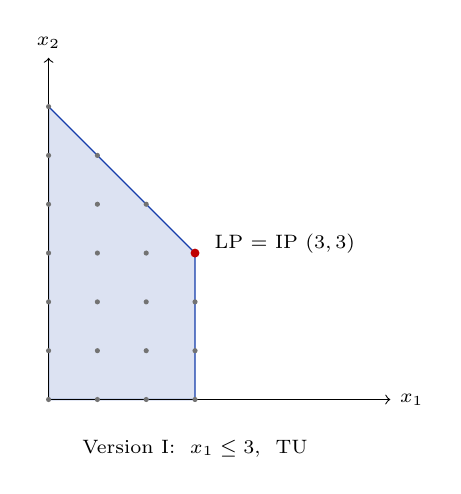
\begin{tikzpicture}[scale=0.62, font=\scriptsize]
  \fill[solink!15] (0,0) -- (3,0) -- (3,3) -- (0,6) -- cycle;
  \draw[solink] (0,0) -- (3,0) -- (3,3) -- (0,6) -- cycle;
  \draw[->] (0,0) -- (7,0) node[right] {$x_1$}; \draw[->] (0,0) -- (0,7) node[above] {$x_2$};
  \foreach \i in {0,1,2,3} \foreach \j in {0,...,6} {\ifnum\numexpr\i+\j\relax<7 \fill[black!55] (\i,\j) circle (1.5pt);\fi}
  \fill[red!75!black] (3,3) circle (2.6pt);
  \node[anchor=west] at (3.2,3.2) {LP $=$ IP $(3,3)$};
  \node at (3,-1) {Version I: \ $x_1 \le 3$, \ TU};
\end{tikzpicture}
\hspace{10mm}
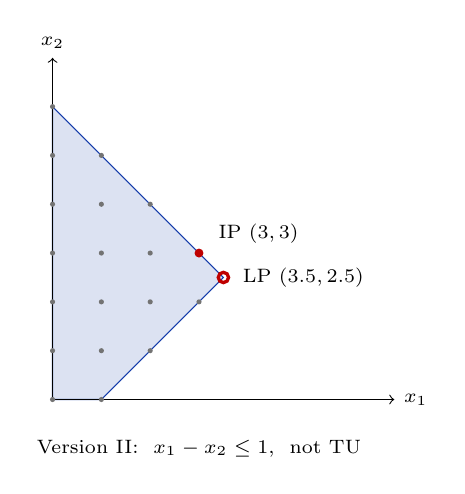
\begin{tikzpicture}[scale=0.62, font=\scriptsize]
  \fill[solink!15] (0,0) -- (1,0) -- (3.5,2.5) -- (0,6) -- cycle;
  \draw[solink] (0,0) -- (1,0) -- (3.5,2.5) -- (0,6) -- cycle;
  \draw[->] (0,0) -- (7,0) node[right] {$x_1$}; \draw[->] (0,0) -- (0,7) node[above] {$x_2$};
  \foreach \p in {(0,0),(1,0),(0,1),(1,1),(2,1),(0,2),(1,2),(2,2),(3,2),(0,3),(1,3),(2,3),(3,3),
                  (0,4),(1,4),(2,4),(0,5),(1,5),(0,6)} \fill[black!55] \p circle (1.5pt);
  \draw[red!75!black, very thick] (3.5,2.5) circle (3pt);
  \fill[red!75!black] (3,3) circle (2.6pt);
  \node[anchor=west] at (3.7,2.5) {LP $(3.5, 2.5)$};
  \node[anchor=west] at (3.2,3.4) {IP $(3,3)$};
  \node at (3,-1) {Version II: \ $x_1 - x_2 \le 1$, \ not TU};
\end{tikzpicture}
\end{center}
$A_{\mathrm{I}}$ is TU, so with integer $b$ every corner is integral and the LP optimum is
the IP optimum --- no gap. $A_{\mathrm{II}}$ is not TU, so nothing guarantees an integral
optimum, and in the figure it is not: the corner where both rows are tight sits at
$(3.5, 2.5)$. Hence the gap.
\end{solution}

\item \textbf{(5 pts)} Keep $A_{\mathrm{II}}$ with integer $b = (b_1, b_2)$,
  $b_1 \ge b_2 \ge 0$. Solve for the corner where both rows are tight; show it is integral
  exactly when $b_1 + b_2$ is even. At $b = (7,1)$ the LP optimum is integral --- does that
  make $A_{\mathrm{II}}$ TU?

\begin{solution}
$x_1 + x_2 = b_1$ and $x_1 - x_2 = b_2$ give
\[
  x_1 = \frac{b_1 + b_2}{2}, \qquad x_2 = \frac{b_1 - b_2}{2} .
\]
$b_1 + b_2$ and $b_1 - b_2$ have the same parity, so both coordinates are integers exactly
when $b_1 + b_2$ is even. At $b = (7,1)$: $x = (4,3)$, integral.

No. TU is a property of $A$ alone --- it has nothing to do with any particular $b$. And the
implication runs one way only: TU guarantees integral corners, but failing TU never
guarantees fractional ones. $b = (7,1)$ is simply a lucky right-hand side on a non-TU
matrix. (That the guarantee really is gone shows at $b = (6,1)$, which returns $(3.5,2.5)$.)
\end{solution}

\item \textbf{(5 pts)} In Version~I, North's real limit is $7$ battery packs at $2$ per
  sortie, and a staff officer writes $x_1 \le 3.5$. Solve the relaxation. Which hypothesis
  of Hoffman--Kruskal fails? Fix the row by rounding.

\begin{solution}
The LP optimum is $(3.5,\, 2.5)$ with $z = 15.5$ --- fractional, even though
$A_{\mathrm{I}}$ is TU. The failed hypothesis is \textbf{$b$ integral}: TU protects you
against every \emph{integer} right-hand side, and $3.5$ is not one.

Rounding: $x_1$ is an integer, so $x_1 \le 3.5 \iff x_1 \le \lfloor 3.5 \rfloor = 3$. The
row becomes $x_1 \le 3$, $b$ is integral again, and the LP returns $(3,3)$, $z = 15$ --- the
IP optimum. Rounding the \emph{bound} is legitimate; rounding the \emph{solution} is what
week 2 warned against.
\end{solution}
\end{parts}

% ================================================================ Problem 3
\problem{20}{Problem 3. Relief convoys}

Trucks move from two sources through a hub to two divisions, whole truckloads only, at
minimum cost; $b = (+9, +5, 0, -8, -6)$ for Port, Airfield, Hub, North, South, with road
costs $(3,7,2,6,2,3,2)$ and capacities $(8,4,5,3,7,6,3)$ on
$(1,3), (1,4), (2,3), (2,5), (3,4), (3,5), (4,5)$.

\begin{parts}
\item \textbf{(3 pts)} Which Week~5 problem models this? Draw the graph and define
  $G = (V,E)$.

\begin{solution}
\textbf{Minimum cost network flow (MCNF)}.
\[
  V = \{1,2,3,4,5\}, \qquad
  E = \{(1,3), (1,4), (2,3), (2,5), (3,4), (3,5), (4,5)\}
\]
\begin{center}
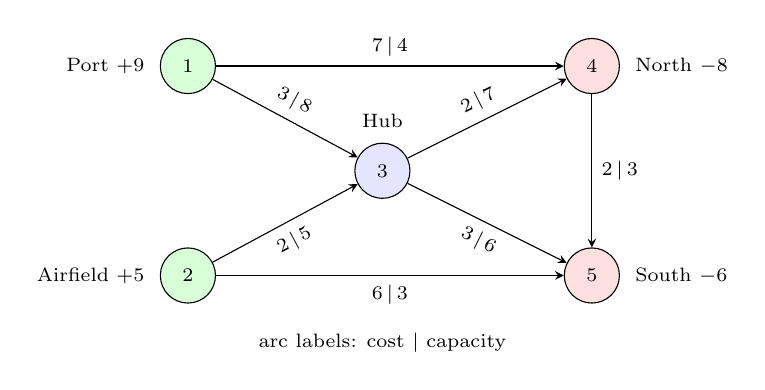
\begin{tikzpicture}[>=stealth, font=\scriptsize, scale=0.95]
  \node[circle, draw, fill=green!15, minimum size=7mm] (n1) at (0,1.4) {1};
  \node[circle, draw, fill=green!15, minimum size=7mm] (n2) at (0,-1.4) {2};
  \node[circle, draw, fill=blue!10,  minimum size=7mm] (n3) at (2.6,0) {3};
  \node[circle, draw, fill=red!12,   minimum size=7mm] (n4) at (5.4,1.4) {4};
  \node[circle, draw, fill=red!12,   minimum size=7mm] (n5) at (5.4,-1.4) {5};
  \node[anchor=east] at (-0.45,1.4) {Port $+9$}; \node[anchor=east] at (-0.45,-1.4) {Airfield $+5$};
  \node[anchor=south] at (2.6,0.45) {Hub};
  \node[anchor=west] at (5.85,1.4) {North $-8$}; \node[anchor=west] at (5.85,-1.4) {South $-6$};
  \draw[->] (n1) -- node[sloped, above] {$3 \,|\, 8$} (n3);
  \draw[->] (n1) -- node[above] {$7 \,|\, 4$} (n4);
  \draw[->] (n2) -- node[sloped, below] {$2 \,|\, 5$} (n3);
  \draw[->] (n2) -- node[below] {$6 \,|\, 3$} (n5);
  \draw[->] (n3) -- node[sloped, above] {$2 \,|\, 7$} (n4);
  \draw[->] (n3) -- node[sloped, below] {$3 \,|\, 6$} (n5);
  \draw[->] (n4) -- node[right] {$2 \,|\, 3$} (n5);
  \node at (2.6,-2.3) {arc labels: cost $|$ capacity};
\end{tikzpicture}
\end{center}
\end{solution}

\item \textbf{(4 pts)} Define $x$; write $A$, $c$, $b$ and their dimensions.

\begin{solution}
$x_a$ = truckloads on arc $a$, one per arc: $x \in \mathbb{R}^{7}$, $c \in \mathbb{R}^{7}$,
$b \in \mathbb{R}^{5}$, and $A \in \mathbb{R}^{5 \times 7}$ is the node--arc incidence matrix
($+1$ where the arc leaves, $-1$ where it arrives). Writing the capacities as rows as well
stacks $I$ underneath:
\[
\binom{A}{I} \;=\;
\bordermatrix{%
  & \scriptstyle (1,3) & \scriptstyle (1,4) & \scriptstyle (2,3) & \scriptstyle (2,5)
  & \scriptstyle (3,4) & \scriptstyle (3,5) & \scriptstyle (4,5) \cr
 \scriptstyle \text{node }1 & +1 & +1 &  0 &  0 &  0 &  0 &  0 \cr
 \scriptstyle \text{node }2 &  0 &  0 & +1 & +1 &  0 &  0 &  0 \cr
 \scriptstyle \text{node }3 & -1 &  0 & -1 &  0 & +1 & +1 &  0 \cr
 \scriptstyle \text{node }4 &  0 & -1 &  0 &  0 & -1 &  0 & +1 \cr
 \scriptstyle \text{node }5 &  0 &  0 &  0 & -1 &  0 & -1 & -1 \cr
 \noalign{\vskip3pt}
 \scriptstyle \text{cap }(1,3) & 1 & 0 & 0 & 0 & 0 & 0 & 0 \cr
 \scriptstyle \text{cap }(1,4) & 0 & 1 & 0 & 0 & 0 & 0 & 0 \cr
 \scriptstyle \text{cap }(2,3) & 0 & 0 & 1 & 0 & 0 & 0 & 0 \cr
 \scriptstyle \text{cap }(2,5) & 0 & 0 & 0 & 1 & 0 & 0 & 0 \cr
 \scriptstyle \text{cap }(3,4) & 0 & 0 & 0 & 0 & 1 & 0 & 0 \cr
 \scriptstyle \text{cap }(3,5) & 0 & 0 & 0 & 0 & 0 & 1 & 0 \cr
 \scriptstyle \text{cap }(4,5) & 0 & 0 & 0 & 0 & 0 & 0 & 1 \cr}
\begin{array}{l}
 \phantom{=\;0} \\
 =\;9 \\ =\;5 \\ =\;0 \\ =\;-8 \\ =\;-6 \\[3pt]
 \le\;8 \\ \le\;4 \\ \le\;5 \\ \le\;3 \\ \le\;7 \\ \le\;6 \\ \le\;3
\end{array}
\]
The top five rows are $Ax = b$, the bottom seven $Ix \le u$; the objective is
$c = (3, 7, 2, 6, 2, 3, 2)^{\top}$.
\end{solution}

\item \textbf{(4 pts)} Explain why $A$ is TU; solve the relaxation and confirm every flow
  is a whole truckload.

\begin{solution}
Checklist: (i) entries are $0, \pm 1$; (ii) every column has exactly two nonzeros, one
$+1$ and one $-1$; (iii) take $M_1 = V$, $M_2 = \emptyset$ --- each column sums to
$(+1) + (-1) = 0$, and the empty sum is $0$. Every node--arc incidence matrix of a directed
graph is TU, with no condition on the graph.
\begin{lstlisting}
import gurobipy as gp
from gurobipy import GRB

arcs = [(1,3), (1,4), (2,3), (2,5), (3,4), (3,5), (4,5)]
cost = dict(zip(arcs, [3, 7, 2, 6, 2, 3, 2]))
cap  = dict(zip(arcs, [8, 4, 5, 3, 7, 6, 3]))
b    = {1: 9, 2: 5, 3: 0, 4: -8, 5: -6}
m = gp.Model("convoys")
x = m.addVars(arcs, lb=0, ub=[cap[a] for a in arcs], name="x")   # continuous
m.setObjective(gp.quicksum(cost[a]*x[a] for a in arcs), GRB.MINIMIZE)
for i in b:                                    # outflow - inflow = b_i
    m.addConstr(gp.quicksum(x[a] for a in arcs if a[0] == i)
                - gp.quicksum(x[a] for a in arcs if a[1] == i) == b[i])
m.optimize()
print("z =", m.ObjVal, {a: x[a].X for a in arcs if x[a].X > 1e-6})
\end{lstlisting}
\begin{lstlisting}
z = 73.0 {(1, 3): 8.0, (1, 4): 1.0, (2, 3): 5.0, (3, 4): 7.0, (3, 5): 6.0}
\end{lstlisting}
Whole truckloads with no integrality declared, as TU promises.
\end{solution}

\item \textbf{(5 pts)} Roads $(1,3)$ and $(3,4)$ share a highway carrying at most $10$
  truckloads. Add it, solve LP and IP, report the gap, and find a $2\times2$ submatrix with
  determinant $\pm 2$.

\begin{solution}
Adding \texttt{m.addConstr(x[1,3] + x[3,4] <= 10)}:
\begin{lstlisting}
LP: z = 78.0 {(1,3): 5.5, (1,4): 3.5, (2,3): 5.0, (3,4): 4.5, (3,5): 6.0}
IP: z = 79.0 {(1,3): 5.0, (1,4): 4.0, (2,3): 5.0, (3,4): 4.0, (3,5): 6.0}
\end{lstlisting}
Gap $= 79 - 78 = 1$, and the LP ships half truckloads.

The highway row joins the five node rows (capacity rows omitted). Permuting rows and columns
changes nothing --- TU and determinants survive reordering --- so put the highway row next to
node~3 and the two shared arcs in the first two columns, and the guilty $2 \times 2$ sits in
plain sight:
\[
\bordermatrix{%
  & \scriptstyle (1,3) & \scriptstyle (3,4) & \scriptstyle (1,4) & \scriptstyle (2,3)
  & \scriptstyle (2,5) & \scriptstyle (3,5) & \scriptstyle (4,5) \cr
 \scriptstyle \text{node }1 & +1 &  0 & +1 &  0 &  0 &  0 &  0 \cr
 \scriptstyle \text{node }2 &  0 &  0 &  0 & +1 & +1 &  0 &  0 \cr
 \scriptstyle \text{node }3 & {\color{red!75!black}-1} & {\color{red!75!black}+1}
   &  0 & -1 &  0 & +1 &  0 \cr
 \scriptstyle \text{highway} & {\color{red!75!black}+1} & {\color{red!75!black}+1}
   &  0 &  0 &  0 &  0 &  0 \cr
 \scriptstyle \text{node }4 &  0 & -1 & -1 &  0 &  0 &  0 & +1 \cr
 \scriptstyle \text{node }5 &  0 &  0 &  0 &  0 & -1 & -1 & -1 \cr}
\begin{array}{l}
 \phantom{=\;0} \\
 =\;9 \\ =\;5 \\ =\;0 \\ \le\;10 \\ =\;-8 \\ =\;-6
\end{array}
\]
The red block is a genuine $2 \times 2$ corner of the matrix:
\[
  \begin{pmatrix} -1 & +1 \\ +1 & +1 \end{pmatrix},
  \qquad \det = -1 - 1 = -2 .
\]
The highway row counts both arcs with $+1$ while node~3 sees one entering and one leaving;
that sign clash is the determinant of $2$, so the matrix is no longer an incidence matrix
and no longer TU.
\end{solution}

\item \textbf{(4 pts)} Instead, the Hub receives at most $10$: split it into Hub-in and
  Hub-out joined by a dock road of capacity $10$. Still TU? Solve. Lesson?

\begin{solution}
The restriction is on the hub's inflow:
\[
  x_{13} + x_{23} \;\le\; 10 .
\]
Written as a row of the matrix it is another (d) --- and column $(1,3)$ would then carry
three nonzeros, so the checklist no longer applies and the guarantee is gone.

Split node 3 instead. Arcs $(1,3_{\mathrm{in}})$, $(2,3_{\mathrm{in}})$ keep their data,
arcs $(3_{\mathrm{out}},4)$, $(3_{\mathrm{out}},5)$ keep theirs, and a dock arc
$(3_{\mathrm{in}}, 3_{\mathrm{out}})$ carries everything through at cost $0$; both new nodes
have $b = 0$. Now \emph{everything} entering the hub must cross the dock, so the same
restriction is simply that arc's capacity,
\[
  0 \;\le\; x_{3_{\mathrm{in}} 3_{\mathrm{out}}} \;\le\; 10 ,
\]
a bound on one variable rather than a row across several.
\begin{center}
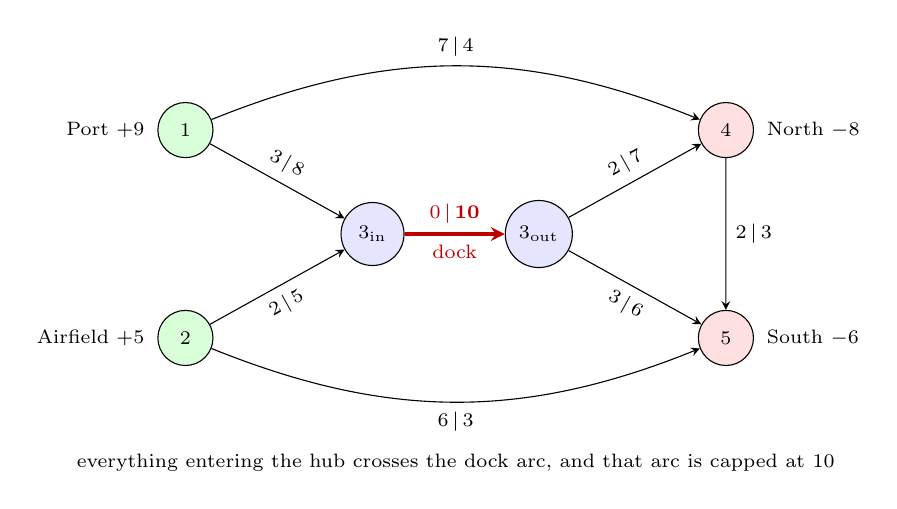
\begin{tikzpicture}[>=stealth, font=\scriptsize, scale=0.88]
  \node[circle, draw, fill=green!15, minimum size=7mm] (n1) at (0,1.5) {1};
  \node[circle, draw, fill=green!15, minimum size=7mm] (n2) at (0,-1.5) {2};
  \node[circle, draw, fill=blue!10,  minimum size=8mm] (hi) at (2.7,0) {$3_{\mathrm{in}}$};
  \node[circle, draw, fill=blue!10,  minimum size=8mm] (ho) at (5.1,0) {$3_{\mathrm{out}}$};
  \node[circle, draw, fill=red!12,   minimum size=7mm] (n4) at (7.8,1.5) {4};
  \node[circle, draw, fill=red!12,   minimum size=7mm] (n5) at (7.8,-1.5) {5};
  \node[anchor=east] at (-0.45,1.5) {Port $+9$}; \node[anchor=east] at (-0.45,-1.5) {Airfield $+5$};
  \node[anchor=west] at (8.25,1.5) {North $-8$}; \node[anchor=west] at (8.25,-1.5) {South $-6$};
  \draw[->] (n1) -- node[sloped, above] {$3 \,|\, 8$} (hi);
  \draw[->] (n2) -- node[sloped, below] {$2 \,|\, 5$} (hi);
  \draw[->, red!75!black, very thick] (hi) -- node[above] {$0 \,|\, \mathbf{10}$} node[below] {dock} (ho);
  \draw[->] (ho) -- node[sloped, above] {$2 \,|\, 7$} (n4);
  \draw[->] (ho) -- node[sloped, below] {$3 \,|\, 6$} (n5);
  \draw[->] (n1) to[bend left=22] node[above] {$7 \,|\, 4$} (n4);
  \draw[->] (n2) to[bend right=22] node[below] {$6 \,|\, 3$} (n5);
  \draw[->] (n4) -- node[right] {$2 \,|\, 3$} (n5);
  \node at (3.9,-3.3) {everything entering the hub crosses the dock arc, and that arc is capped at $10$};
\end{tikzpicture}
\end{center}
\begin{lstlisting}
LP: z = 76.0 {(1,3in): 8.0, (1,4): 1.0, (2,3in): 2.0, (2,5): 3.0,
              (3in,3out): 10.0, (3out,4): 7.0, (3out,5): 3.0}
IP: z = 76.0   (identical)
\end{lstlisting}
Still TU --- it is again a node--arc incidence matrix, just of a bigger graph --- so the LP
is integral and the dock arc sits at its capacity, $10$.

(The side-row version happens to return $76$ integral on this data too. That is 2(c)'s point
again: without the structure you have no promise, only luck.)

\textbf{Lesson:} as long as every row is still a flow-conservation row, adding nodes and arcs
does not destroy TU --- the matrix is simply the incidence matrix of a bigger graph --- so the
LP relaxation is still guaranteed to solve the IP.
\end{solution}
\end{parts}

% ================================================================ Problem 4
\problem{20}{Problem 4. The LAP}

Bases 1 (North) and 2 (South) may hold a reserve for town 3 ($d_3 = 8$) and village 4
($d_4 = 4$); $f_1 = 20$, $f_2 = 16$; roads $c_{13} = 2$, $c_{23} = 4$, $c_{24} = 1$,
$c_{34} = 1$, $c_{43} = 2$; $h_i = 1$, $u_i = 40$, $o_i = 1$, $B = 16$, $p = 1$.

\begin{parts}
\item \textbf{(5 pts)} Write the LAP for this instance with numbers.

\begin{solution}
\[
\begin{aligned}
  \min\quad & 20 x_1 + 16 x_2 + r_1 + r_2
            + 2 y_{13} + 4 y_{23} + y_{24} + y_{34} + 2 y_{43}
            + 40(q_3 + q_4) + \textstyle\sum_i s_i \\
  \text{s.t.}\quad
   & -y_{13} + r_1 + q_1 - s_1 = 0 && \text{[node 1]} \\
   & -y_{23} - y_{24} + r_2 + q_2 - s_2 = 0 && \text{[node 2]} \\
   & y_{13} + y_{23} + y_{43} - y_{34} + q_3 - s_3 = 8 && \text{[node 3]} \\
   & y_{24} + y_{34} - y_{43} + q_4 - s_4 = 4 && \text{[node 4]} \\
   & r_1 + r_2 \le 16, \qquad r_1 \le 16 x_1, \qquad r_2 \le 16 x_2, \qquad x_1 + x_2 \le 1 \\
   & y, r, s \ge 0, \quad 0 \le q_i \le d_i \ \ (\text{so } q_1 = q_2 = 0), \quad x_1, x_2 \in \{0,1\}
\end{aligned}
\]
\end{solution}

\item \textbf{(5 pts)} Which entries break TU? Show that once $x$ is fixed the rest is TU.

\begin{solution}
The linking rows $r_i \le 16 x_i$ carry the entry $-16$ (as $r_i - 16x_i \le 0$). A TU
matrix may only contain $0, \pm 1$.

Therefore, with $x$ fixed, $16 x_i$ is just an integer bound on $r_i$, and the remaining
constraints are a network. Give the budget row a slack $t \ge 0$ and read it as the
conservation row of one extra \emph{depot} node $0$ that feeds $r_1$ and $r_2$. Order the
free variables as
\[
  \mathbf{x} \;=\; (\,r_1,\; r_2,\; t,\; y_{13},\; y_{23},\; y_{24},\; y_{34},\; y_{43},\;
                     q_3,\; q_4,\; s_1,\; s_2,\; s_3,\; s_4\,)^{\top}
\]
($q_1 = q_2 = 0$ because $d_1 = d_2 = 0$). Writing every row as outflow $-$ inflow:
\[
\bordermatrix{%
  & \scriptstyle r_1 & \scriptstyle r_2 & \scriptstyle t & \scriptstyle y_{13}
  & \scriptstyle y_{23} & \scriptstyle y_{24} & \scriptstyle y_{34} & \scriptstyle y_{43}
  & \scriptstyle q_3 & \scriptstyle q_4 & \scriptstyle s_1 & \scriptstyle s_2
  & \scriptstyle s_3 & \scriptstyle s_4 \cr
 \scriptstyle \text{depot} & +1 & +1 & +1 &  0 &  0 &  0 &  0 &  0 &  0 &  0 &  0 &  0 &  0 &  0 \cr
 \scriptstyle \text{node }1 & -1 &  0 &  0 & +1 &  0 &  0 &  0 &  0 &  0 &  0 & +1 &  0 &  0 &  0 \cr
 \scriptstyle \text{node }2 &  0 & -1 &  0 &  0 & +1 & +1 &  0 &  0 &  0 &  0 &  0 & +1 &  0 &  0 \cr
 \scriptstyle \text{node }3 &  0 &  0 &  0 & -1 & -1 &  0 & +1 & -1 & -1 &  0 &  0 &  0 & +1 &  0 \cr
 \scriptstyle \text{node }4 &  0 &  0 &  0 &  0 &  0 & -1 & -1 & +1 &  0 & -1 &  0 &  0 &  0 & +1 \cr}
\begin{array}{l}
 \phantom{=\;0} \\
 =\;16 \\ =\;0 \\ =\;0 \\ =\;-8 \\ =\;-4
\end{array}
\]
with $0 \le r_i \le 16 x_i$, $0 \le q_i \le d_i$, and $y, s, t \ge 0$.

Every column has at most two nonzeros, and every column that has two carries one $+1$ and
one $-1$ --- a node--arc incidence matrix, hence TU. The right-hand side is integer, so the
LP relaxation solves the IP.
\end{solution}

\item \textbf{(6 pts)} Solve the IP and its relaxation; report both plans and the gap. Then
  fix $x$ at the IP's value and solve the LP again.

\begin{solution}
\begin{lstlisting}
IP : z = 56.0  x = {1: 0, 2: 1}   r = {2: 12.0}   y = {(2,4): 12.0, (4,3): 8.0}
LP : z = 46.0  x = {1: 0.5, 2: 0.25}  r = {1: 8.0, 2: 4.0}  y = {(1,3): 8.0, (2,4): 4.0}
\end{lstlisting}
Gap $= 56 - 46 = 10$.

The IP opens South only ($16$), stocks $12$\,t ($12$), ships all $12$ to the village and
$8$ of it onward to the town: $12 \cdot 1 + 8 \cdot 2 = 28$. Total $16 + 12 + 28 = 56$.

The LP opens \emph{half} of North and a \emph{quarter} of South, which buys the cheapest
roads from both ($8$\,t town from North at $2$, $4$\,t village from South at $1$) while
paying only $20 \cdot \tfrac12 + 16 \cdot \tfrac14 = 14$ at the door. That is the big-$M$
leak: $r_i \le 16 x_i$ lets $x_i = r_i/16$ unlock the stock for a fraction of the opening cost.

Fixing $x = (0,1)$ and re-solving the LP returns $z = 56$ with the integral plan above: with
$x$ fixed the model is the network of part (b), TU with integer data, so its LP optimum is
integral. All the fractionality lived in $x$.
\end{solution}

\item \textbf{(4 pts)} Which variables are stage~1 and which stage~2? Keep the IP's stage-1
  decisions, let the town's demand be $10$\,t, and solve stage~2.

\begin{solution}
\textbf{Stage 1} (before the demand is known): $x_i$, $r_i$. \quad
\textbf{Stage 2} (after): $y_{ij}$, $q_i$, $s_i$.

Stage 1 is frozen at $x = (0,1)$, $r_2 = 12$, costing $16 + 12 = 28$. With $d_3 = 10$ total
demand is $14 > 12$, so $2$\,t must go short:
\begin{lstlisting}
stage 2: z = 108.0  y = {(2,4): 12.0, (4,3): 8.0}  q = {3: 2.0}
total = 28 + 108 = 136
\end{lstlisting}
The shortage lands at the \textbf{town}: both nodes pay the same $40$/t penalty, so the
model shorts wherever delivery is \emph{dearest} --- the town costs $1 + 2 = 3$/t to reach
through the village, the village $1$/t, so shorting the town saves $3$ and shorting the
village only $1$. Recourse $= 12 \cdot 1 + 8 \cdot 2 + 2 \cdot 40 = 108$.
\end{solution}
\end{parts}

% ================================================================ Problem 5
\problem{20}{Problem 5. Strong vs weak linking}

Depots D1, D2, D3 and brigades B1, B2, B3 on a ring; each brigade is served by its two
neighbours. $y_{ij}$ = fraction of B$j$'s demand from D$i$; costs per ton $c_{ij}$ with
$c_{11} = 1$, $c_{21} = 2$, $c_{22} = 1$, $c_{32} = 2$, $c_{33} = 1$, $c_{13} = 2$;
demands $4, 5, 6$; opening costs $20, 16, 18$.

\begin{parts}
\item \textbf{(5 pts)} Write the strong and weak formulations. What is the smallest valid
  $M$?

\begin{solution}
Both share
$\min \sum_i f_i x_i + \sum_{ij} c_{ij} d_j y_{ij}$ s.t.\ $\sum_{i} y_{ij} = 1$ for every
brigade $j$, $y \ge 0$, $x \in \{0,1\}^3$, and differ only in the linking:
\[
  \text{(strong)} \ \ y_{ij} \le x_i \ \ \text{for each road } (i,j)
  \qquad\qquad
  \text{(weak)} \ \ \textstyle\sum_{j} y_{ij} \le M x_i \ \ \text{for each depot } i .
\]
Each depot serves exactly two brigades and each $y_{ij} \le 1$, so
$\sum_j y_{ij} \le 2$ and the smallest valid $M$ is $\mathbf{M = 2}$.
\end{solution}

\item \textbf{(4 pts)} Prove the strong formulation is better, with the two-step recipe.

\begin{solution}
\emph{Step 1 --- $P_{\mathrm{strong}} \subseteq P_{\mathrm{weak}}$.} Sum the two strong rows
at depot $i$: $\sum_j y_{ij} \le 2 x_i = M x_i$, which is the weak row. So every strong-feasible
point is weak-feasible.

\emph{Step 2 --- the inclusion is strict.} Take $x = (\tfrac12, \tfrac12, \tfrac12)$,
$y_{11} = y_{22} = y_{33} = 1$, all other $y = 0$. Weak holds: $\sum_j y_{1j} = 1 \le 2 \cdot \tfrac12$.
Strong fails: $y_{11} = 1 > x_1 = \tfrac12$. So $P_{\mathrm{strong}} \subsetneq P_{\mathrm{weak}}$,
and minimizing over the smaller set can only give a larger (better) lower bound.
\end{solution}

\item \textbf{(6 pts)} Solve the IP and both relaxations; verify
  $z_{\mathrm{LP}}^{\text{weak}} \le z_{\mathrm{LP}}^{\text{strong}} \le z_{\mathrm{IP}}$.

\begin{solution}
\begin{lstlisting}
import gurobipy as gp
from gurobipy import GRB

pairs = {1: [1, 2], 2: [2, 3], 3: [3, 1]}        # brigade j -> its two depots
c = {(1,1):1, (2,1):2, (2,2):1, (3,2):2, (3,3):1, (1,3):2}
d = {1: 4, 2: 5, 3: 6};  f = {1: 20, 2: 16, 3: 18}

def solve(kind, binary):
    m = gp.Model(); m.Params.OutputFlag = 0
    vt = GRB.BINARY if binary else GRB.CONTINUOUS
    x = m.addVars([1,2,3], vtype=vt, lb=0, ub=1)
    y = m.addVars(c.keys(), lb=0, ub=1)
    m.setObjective(gp.quicksum(f[i]*x[i] for i in [1,2,3])
                   + gp.quicksum(c[k]*d[k[1]]*y[k] for k in c), GRB.MINIMIZE)
    m.addConstrs(gp.quicksum(y[(i,j)] for i in pairs[j]) == 1 for j in [1,2,3])
    if kind == "strong":
        m.addConstrs(y[k] <= x[k[0]] for k in c)
    else:
        m.addConstrs(gp.quicksum(y[(i,j)] for j in [1,2,3] if (i,j) in c) <= 2*x[i]
                     for i in [1,2,3])
    m.optimize()
    return m.ObjVal, {i: round(x[i].X, 3) for i in [1,2,3]}

for k in ("weak", "strong"):
    print(k, "LP:", solve(k, False))
print("IP    :", solve("strong", True))
\end{lstlisting}
\begin{lstlisting}
weak LP: (42.0, {1: 0.5, 2: 0.5, 3: 0.5})
strong LP: (49.5, {1: 0.5, 2: 0.5, 3: 0.5})
IP    : (53.0, {1: 0.0, 2: 1.0, 3: 1.0})
\end{lstlisting}
$42 \le 49.5 \le 53$ as required. The IP opens D2 and D3 and serves B1 from D2.

The \textbf{strong} bound is the useful one: it leaves a gap of $3.5$ against the weak
formulation's $11$, on the same integer feasible set. Same answers, a bound three times
tighter --- and the bound is what branch \& bound spends its time on.
\end{solution}

\item \textbf{(5 pts)} Derive $x_i + x_{i'} \ge 1$ for each brigade's two depots; which
  $3 \times 3$ matrix is this? Add them, divide by $2$ and round up: does the cut close the
  gap?

\begin{solution}
Brigade $j$ needs $y_{ij} + y_{i'j} = 1$ and the strong rows give $y_{ij} \le x_i$,
$y_{i'j} \le x_{i'}$, so $x_i + x_{i'} \ge 1$ --- one of each brigade's two neighbours must
open. The three rows are
\[
  \begin{pmatrix} 1&1&0 \\ 0&1&1 \\ 1&0&1 \end{pmatrix}, \qquad \det = 2 ,
\]
the incidence matrix of the \textbf{triangle} --- week 5's odd cycle, the non-bipartite case
that fails the checklist. Not TU, which is exactly why the LP can sit at
$x = (\tfrac12,\tfrac12,\tfrac12)$: every row reads $\tfrac12 + \tfrac12 = 1$, so adding
these three rows alone changes nothing (the strong LP stays at $49.5$).

Add them up: $2(x_1 + x_2 + x_3) \ge 3$, divide by $2$, and round the right-hand side up
because $\sum_i x_i$ is an integer:
\[
  \textstyle\sum_i x_i \;\ge\; \lceil 1.5 \rceil \;=\; 2 .
\]
This one cuts off $(\tfrac12,\tfrac12,\tfrac12)$, and the strong LP jumps to
$z = 53$ with $x = (0,1,1)$ --- \textbf{the gap closes completely}. (On the weak
formulation the same cut only reaches $50$: a cut helps, but it cannot repair a bad
formulation.)
\end{solution}
\end{parts}

\end{document}
